\chapter{Das Spiel FeedMe}
Angelina Scheler

\section{Der Entwurf}

Die Idee von FeedMe war es Multiple Choice Fragen interessanter zu gestalten, damit die Schüler motiviert bleiben. Eigenschaften des Spiels:

\begin{itemize}
\item Multiple Choice
\item für alle Fächer geeignet
\item Monster muss mit richtiger Antwort gefüttert
\item bei falscher Antwort wird ein Leben abgezogen
\item verliert der Spieler zu viele Leben, wird das Monster wütend
\end{itemize}

\begin{figure}[H]
	\centering
  \frame{ 
  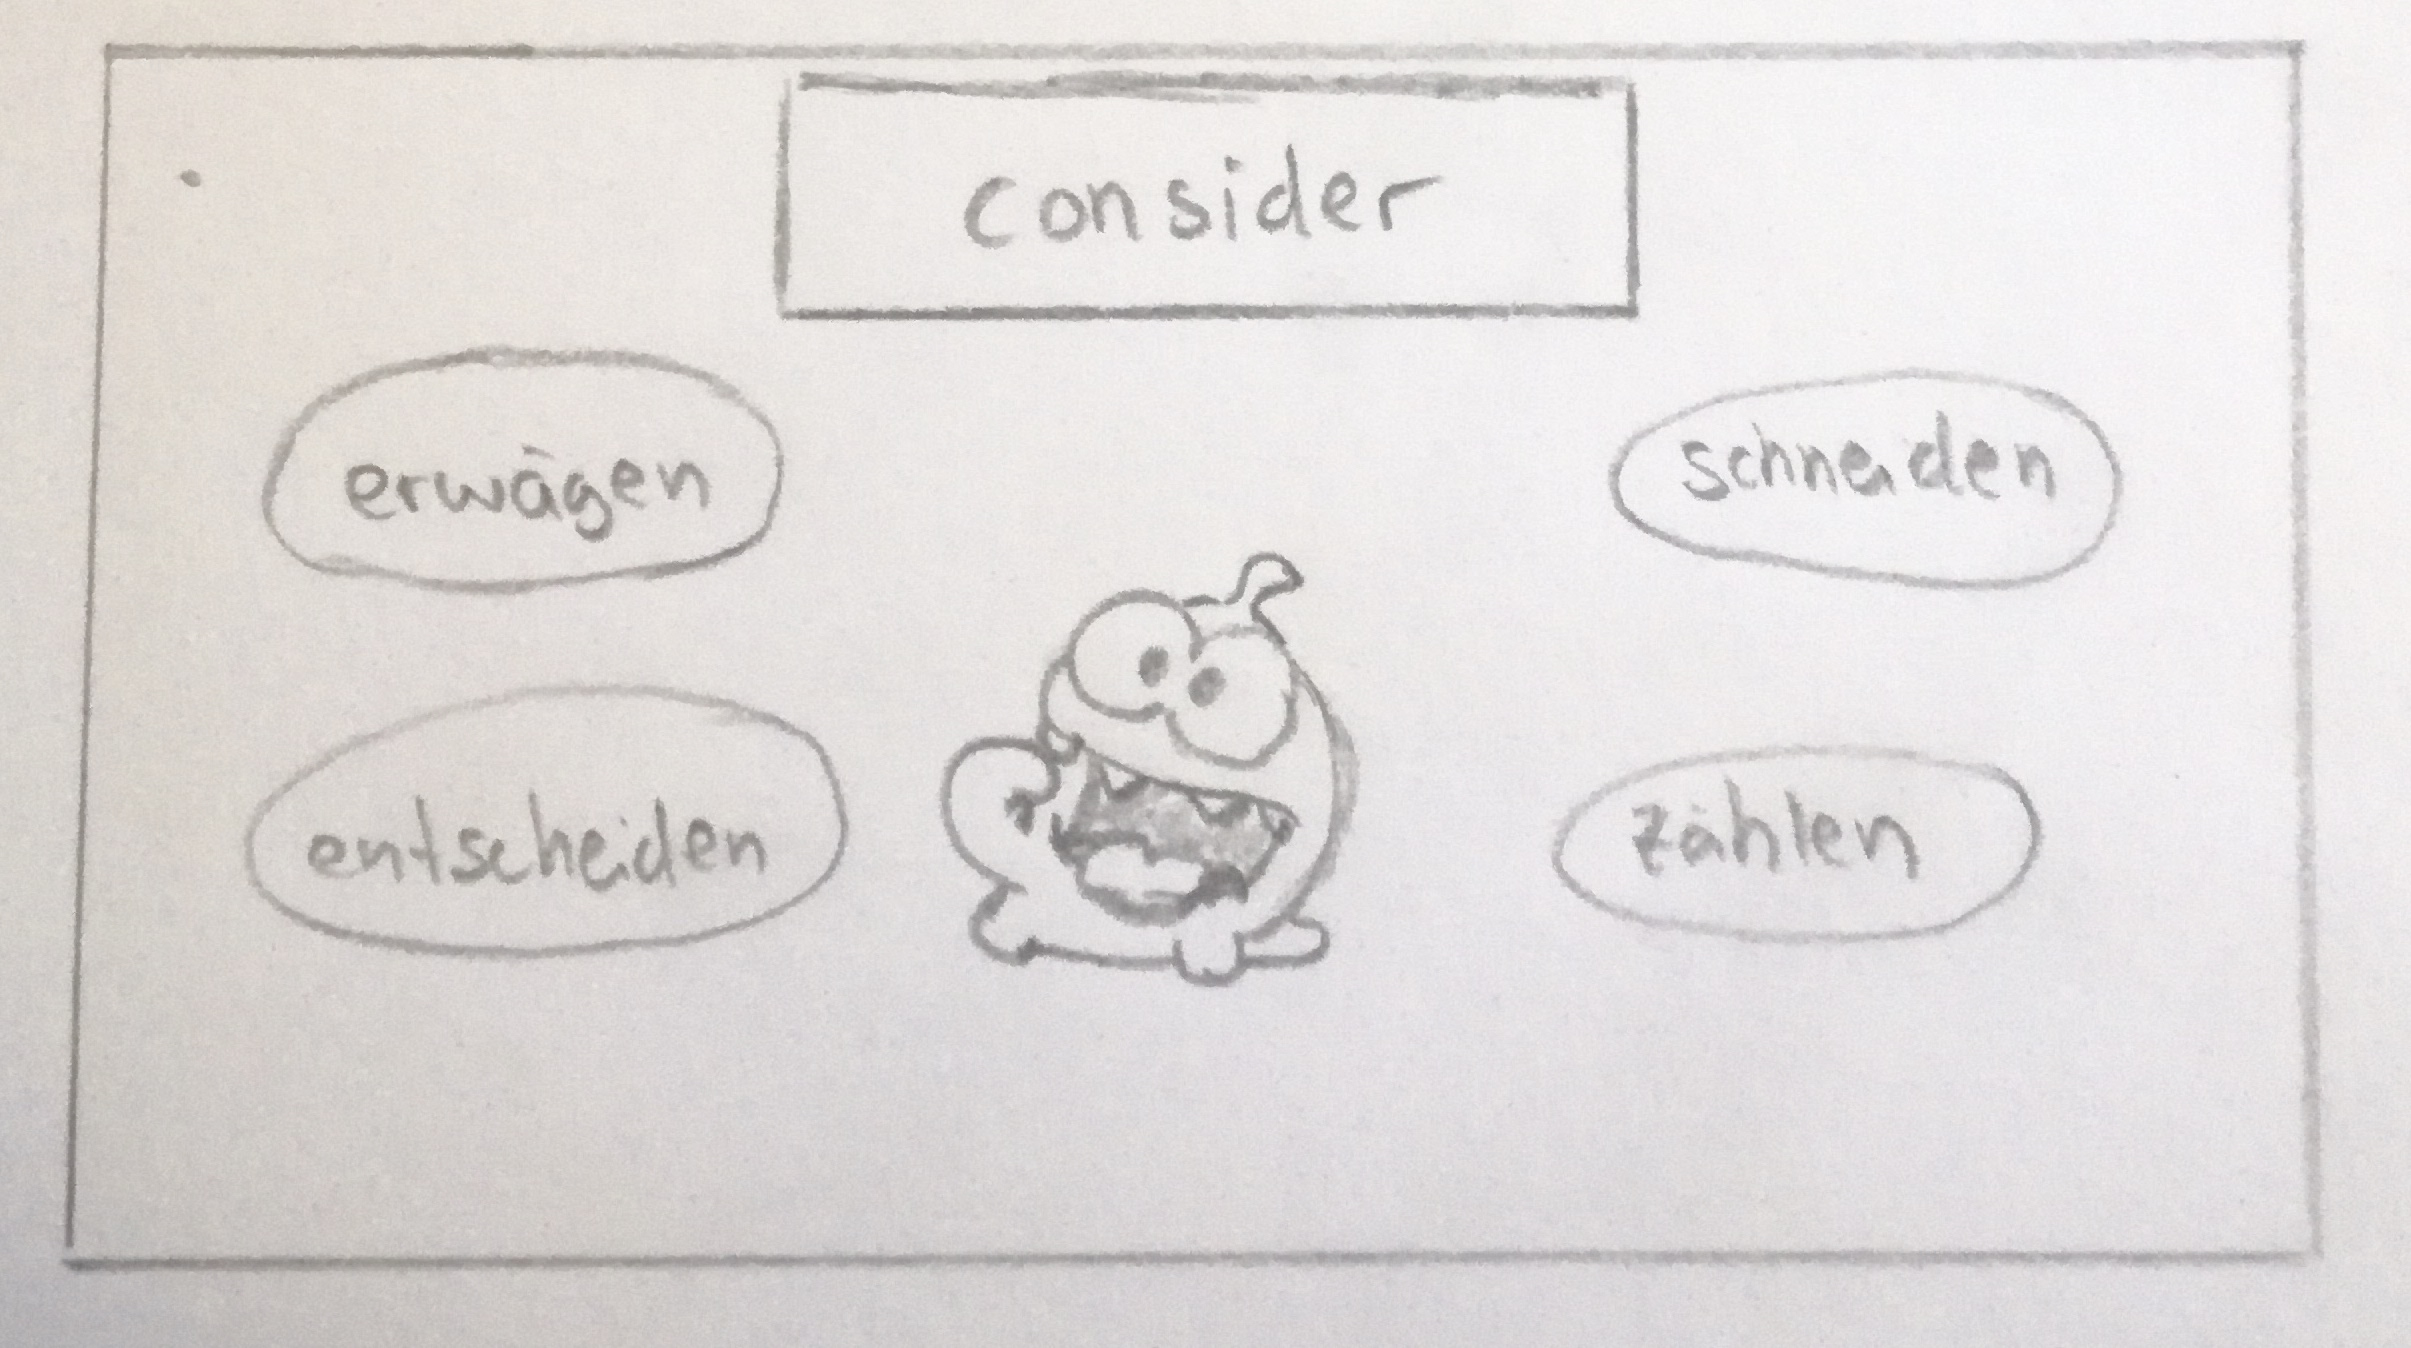
\includegraphics[width=0.99\textwidth]{images/FeedMeEntwurf.jpg}
  }
	\caption{Erster Entwurf}
	\label{Erster Entwurf}
\end{figure}



\section{Die Umsetzung und Implementierung}

Das Spiel wurde mit dem SpriteKit umgesetzt
\begin{figure}[H]
	\centering
  \frame{ 
  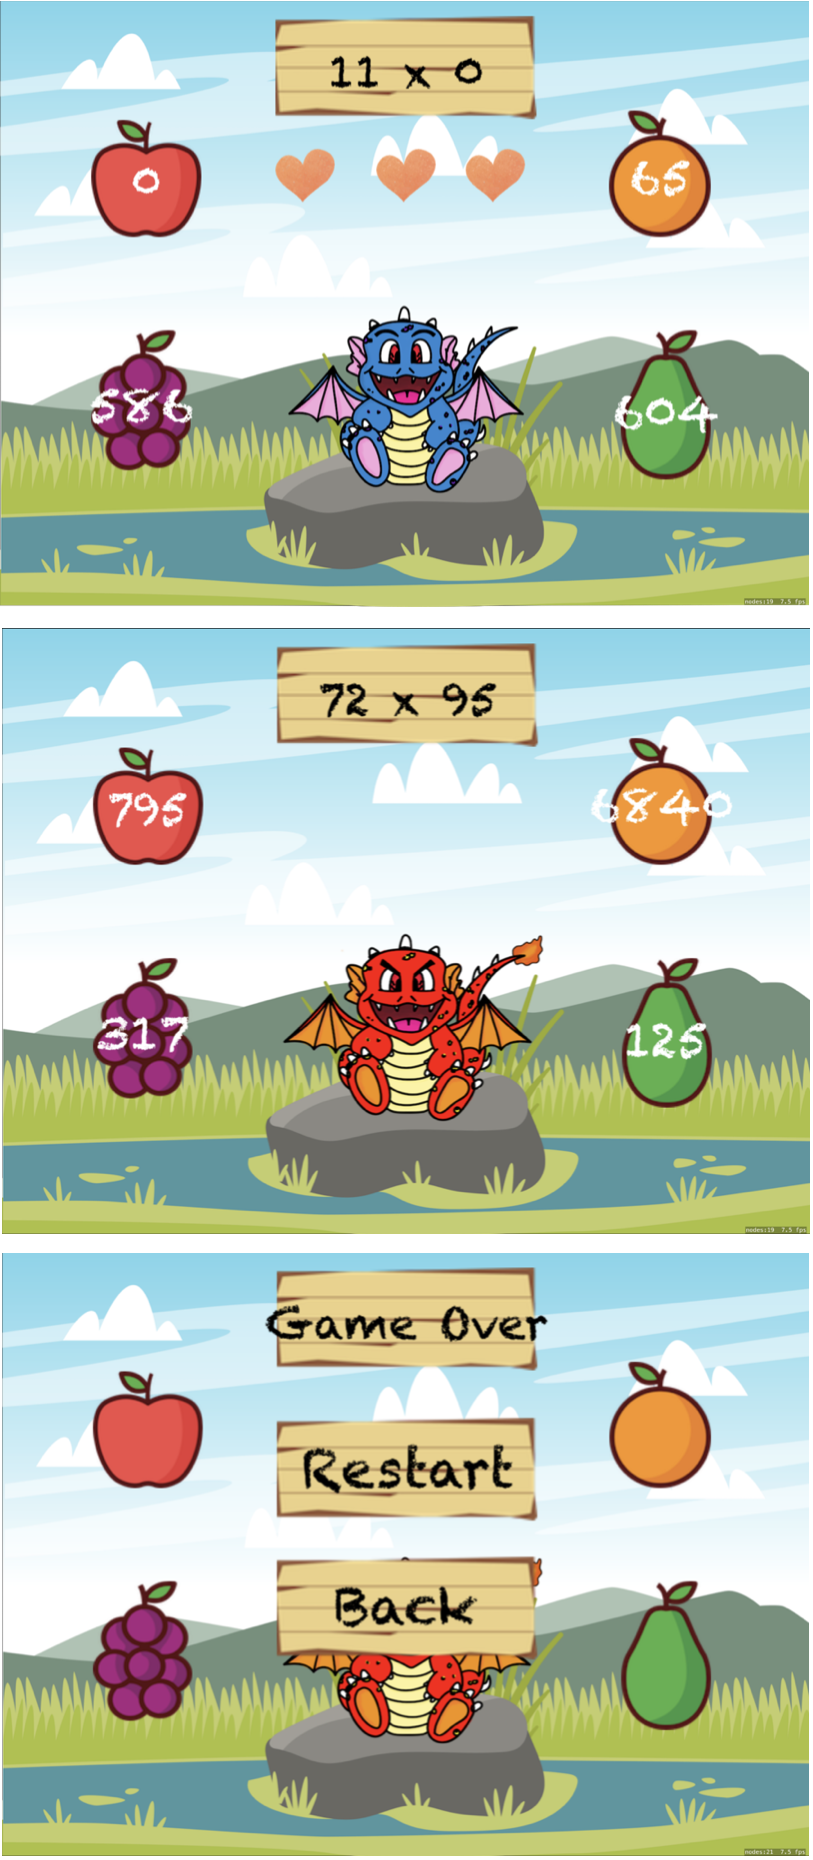
\includegraphics[width=0.6\textwidth]{images/FeedMeScreens.png}
  }
	\caption{Game Screens}
	\label{Game Screens}
\end{figure}


In einem SpriteKit Scene File wurden Color Sprites und Labels als Nodes eingefügt, den Sprites Assets zugewiesen, Skalierung und Position angepasst. (GameFeedMeScene.sks)
In \textit{GameFeedMeSwift.swift} wurden dann die Funktion umgesetzt.

\subsection{Die Nodes}
Für alle benötigten Nodes aus der Scene wurden Variablen angelegt z.B.

		\textit{var frage: SKLabelNode?}

und in der didMove() Methode initialisiert z. B.

		\textit{self.frage = question?.childNode(withName: "frage") as? SKLabelNode}

\subsection{Der Sound}
Über ein SKAudioNode wird der Sound initialisiert. Hintergrundmusik, Touch, falsche/richtige Antwort, Game Over und New Game.
Beispielsweise die Hintergrundmusik als Loop in der didMove() Methode

\textit{let backgroundMusic = SKAudioNode(fileNamed: "sky-loop.wav")
        backgroundMusic.autoplayLooped = true
        addChild(backgroundMusic)}

und beim Bewegen der „Früchte“ als einmaliger Ton in touchesBegan()

\textit{run(SKAction.playSoundFileNamed("beeps.wav", waitForCompletion: false))}

\subsection{Die Touch-Events}
Um die Antworten bewegen zu können sind 3 Funktionen nötig:

\begin{itemize}
\item touchesBegan()
\item touchesMoved()
\item touchesEnded()
\end{itemize}

In der touchesBegan() Funktion wird eine location variable initialisiert, welche die Postion des „touch“ enthält. 
Befindet sich die location auf einer der Antworten wird einer Hilfsvariable „movableNode“ die Postion zugewiesen und die ursprüngliche Position in einer weiteren Hilfsvariable „originalposition“ zwischengespeichert und in der touchesMoved() Funktion ständig aktualisiert. 
Endet das Touch Event wird in der touchesEnded() Methode das „movableNode“ an die „originalPosition“ verwiesen und „movablenode“ zurückgesetzt.

\begin{figure}[H]
	\centering
  \frame{ 
  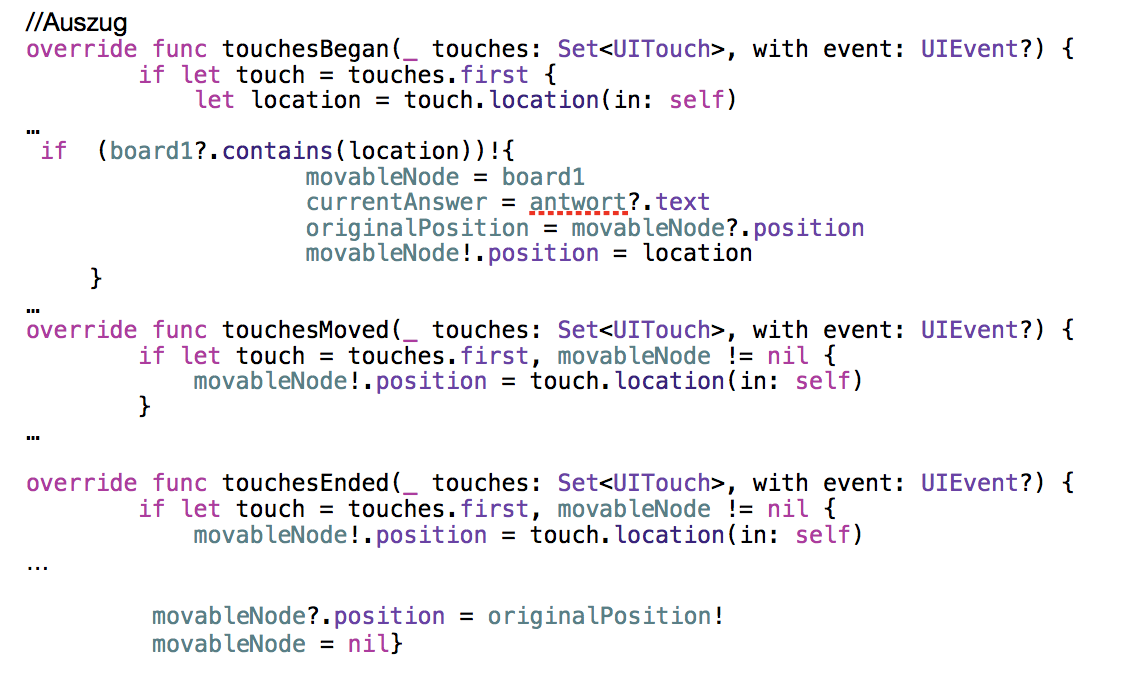
\includegraphics[scale=0.7]{images/FeedMeTouch.png}
  }
	\caption{Die Touch-Events}
	\label{Die Touch-Events}
\end{figure}




\subsection{Die Animation}

Der Drache wurde über eine SKAction animiert. Zunächst wurde ein Images.Atlas Ordner mit verschiedenen Bildern des Drachens angelegt.

\begin{figure}[H]
	\centering
  \frame{ 
  
\includegraphics[scale=0.7]{images/FeedMeDragons.png}
  }
	\caption{Drachen Assets}
	\label{Drachen Assets}
\end{figure}

Die Bilder wurden in ein SKTexture Array „dragonFrames“ bzw. „evilDragonFrames in der buildDragon() Funktion eingelesen. 
In der animateDragon() Funktion wird über dragon.run auf das Array zugegriffen und über ein Zeitintervall die Frames des SKSpriteNode des Drachen geändert.

	\textit{dragon?.run(SKAction.repeatForever(
                	SKAction.animate(with: dragonFrames,
                                 	timePerFrame: 0.5,
                                	 resize: false,
                                	 restore: true)),
                       	 withKey:“walkingInPlaceDragon")}
                        
                        

Die Leben in Form von Herzen(siehe. Abb. GameScreen) werden ebenfalls über eine SKAction animiert.

	einblenden über „fadeIn()“
	\textit{heart?.run(SKAction.fadeIn(withDuration: 2.0))}
	
	ausblenden über „fadeOut()“
	\textit{heart?.run(SKAction.fadeOut(withDuration: 1.0))}
	
	mit „withDuration“, kann die Geschwindigkeit angegeben werden
	
	

\subsection{Das Game Play}

Der User startet mit 3 Leben welche durch die Herzen angezeigt wird, durch ziehen der „Früchte“ auf den Drachen wird die Antwort geprüft, bei falscher Antwort verliert der User ein Leben, befindet er sich kurz vor dem „Game Over“ ändert der Drache die Farbe „wird böse“.

Durch initialisieren eines Integer Arrays welches 4 zufällige Zahlen enthält, werden die Frage, die Antworten generiert und die Antworten den Nodes zufällig zugeordnet.

Ist der User „Game Over“ bzw. hat alle Leben verloren, kann er entweder das Spiel Neustarten oder dieses Beenden über den jeweiligen Button.


